% Uncomment for handout
%\def\HANDOUT{}


\ifdefined\HANDOUT
\documentclass[handout]{beamer}
\usepackage{pgfpages}
\pgfpagesuselayout{4 on 1}[letterpaper,landscape,border shrink=5mm]
\else
\documentclass{beamer}
\fi

\mode<presentation>
{
  \usetheme{Warsaw}
  \definecolor{sered}{rgb}{0.78, 0.06, 0.18}
  \definecolor{richblack}{rgb}{0.0, 0.0, 0.0}
  \setbeamercolor{structure}{fg=sered,bg=richblack}
  %\setbeamercovered{transparent}
}


\usepackage[english]{babel}
\usepackage[latin1]{inputenc}
\usepackage{times}
\usepackage[T1]{fontenc}
\usepackage{tikz}
\usepackage{graphicx}
\usepackage[export]{adjustbox}
\usepackage{fancyvrb}
\usepackage{amsmath}
\usepackage{amssymb}
\usepackage{esvect}

\makeatletter
\newcommand{\imagesource}[1]{{\centering\hfill\break\hbox{\scriptsize Image Source:\thinspace{\tiny\itshape #1}}\par}}
\newcommand{\image}[3][\@nil]{%
        \def\tmp{#1}%
        \begin{center}
        \ifx\tmp\@nnil
            \includegraphics[max height = 0.55\textheight, max width = \textwidth]{images/#2}
        \else
            \includegraphics[max height = 0.50\textheight, max width = \textwidth]{images/#2}
            \linebreak
            #1
        \fi
        \linebreak
        {\tiny Image Source:\thinspace{\tiny #3}}
        \end{center}
}

\newenvironment{code}{%
 \VerbatimEnvironment
 \begin{adjustbox}{max width=\textwidth, max height=0.7\textheight}
 \begin{BVerbatim}
  }{
  \end{BVerbatim}
 \end{adjustbox}
}

\title{Discussion Tracking Application}


\author{Robert Lowe}

\institute[Southeast Missouri State University] % (optional, but mostly needed)
{
  Department of Computer Science\\
  Southeast Missouri State University
}

\date[]{}
\subject{}

\pgfdeclareimage[height=1.0cm]{university-logo}{images/semo-logo}
\logo{\pgfuseimage{university-logo}}



\AtBeginSection[]
{
  \begin{frame}<beamer>{Outline}
    \tableofcontents[currentsection]
  \end{frame}
}


\begin{document}

\begin{frame}
  \titlepage
\end{frame}

\begin{frame}{Outline}
  \tableofcontents
\end{frame}


% Structuring a talk is a difficult task and the following structure
% may not be suitable. Here are some rules that apply for this
% solution: 

% - Exactly two or three sections (other than the summary).
% - At *most* three subsections per section.
% - Talk about 30s to 2min per frame. So there should be between about
%   15 and 30 frames, all told.

% - A conference audience is likely to know very little of what you
%   are going to talk about. So *simplify*!
% - In a 20min talk, getting the main ideas across is hard
%   enough. Leave out details, even if it means being less precise than
%   you think necessary.
% - If you omit details that are vital to the proof/implementation,
%   just say so once. Everybody will be happy with that.

\section{General Procedure}
\begin{frame}{Basic Tensor Analysis Procedure}
    \begin{columns}
    \column{0.5\textwidth}
    
    \begin{enumerate}
        \item Prepare Data
        \item Encode Data as Tensors
        \item Perform Decompositions
        \item Interpret Factors
    \end{enumerate}
    
    \column{0.5\textwidth}
    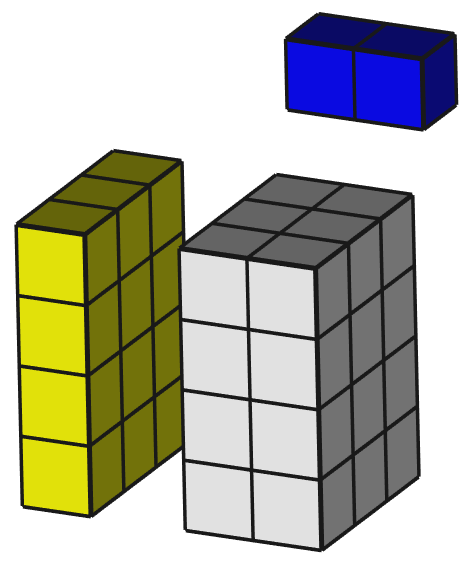
\includegraphics[max width=\textwidth, max height=0.7\textheight]{images/tensor}
    \end{columns}
\end{frame}

\begin{frame}{Encoding}
    \[
    x_{i_1,i_2,\ldots,i_n} \in \mathcal{X}
    \]
    
    \begin{itemize}
        \item Suppose we have an $n$ mode tensor.
        \item What does each mode represent?
        \item Clearly define what the values at each index represent.
        \item Commonly
        \begin{itemize}
            \item Frequncy Counts
            \item Measurements
            \item Color Values
        \end{itemize}
    \end{itemize}
\end{frame}

\begin{frame}{Interpretation}
    \begin{itemize}
        \item What does each factor tell you?
        \item How do factors relate to factors of other tensors?
        \item What features are you looking for?
        \item What classifications can you make?
    \end{itemize}
\end{frame}

\section{Enron Discussion Tracking}
\begin{frame}{Source Paper}
   Bader, Brett W., Michael W. Berry, and Murray Browne. \textit{Discussion tracking in Enron email using PARAFAC}. In Survey of Text Mining II, pp. 147-163. Springer, London, 2008. 
\end{frame}

\begin{frame}{Enron Scandal}
    \begin{columns}
    \column{0.5\textwidth}
    \begin{itemize}
        \item In 2001, accounting irregularities came to light in Enron.
        \item The company eventually filed for bankruptcy.
        \item Part of the discovery process made Enron corporate emails part of the public record. (A goldmine for data scientists!)
    \end{itemize}
    \column{0.5\textwidth}
    \image[Enron Logo]{enron-logo}{\href{https://en.wikipedia.org/wiki/Enron_scandal}{Wikipedia}}
    \end{columns}
\end{frame}

\begin{frame}{Tensor Encoding}
    \[
    \mathrm{term} \times \mathrm{author} \times \mathrm{month}
    \]
    \[
        m \times n \times p
    \]
    \[
    69,157 \times 197 \times 12
    \]
    \begin{columns}
    \column{0.5\textwidth}
    \begin{itemize}
        \item $m$ terms
        \item $n$ authors
        \item $p$ months
    \end{itemize}
    \column{0.5\textwidth}
    \[
        x_{i,j,k}
    \]
    Weight of term according to:
    \begin{itemize}
        \item Term $i$ 
        \item Author $j$
        \item Month $k$
    \end{itemize}
    \end{columns}
\end{frame}

\begin{frame}{Tensor Decompositions}
    \begin{itemize}
        \item Decomposed at rank 25.
        \item Decomposed with both PARAFAC and Non-Negative PARAFAC.
        \item Each factor contains terms and authors over months.
        \item The 25 factors were categorized according to their terms, where possible.
    \end{itemize}
\end{frame}

\begin{frame}{PARAFAC Results}
    \begin{center}
    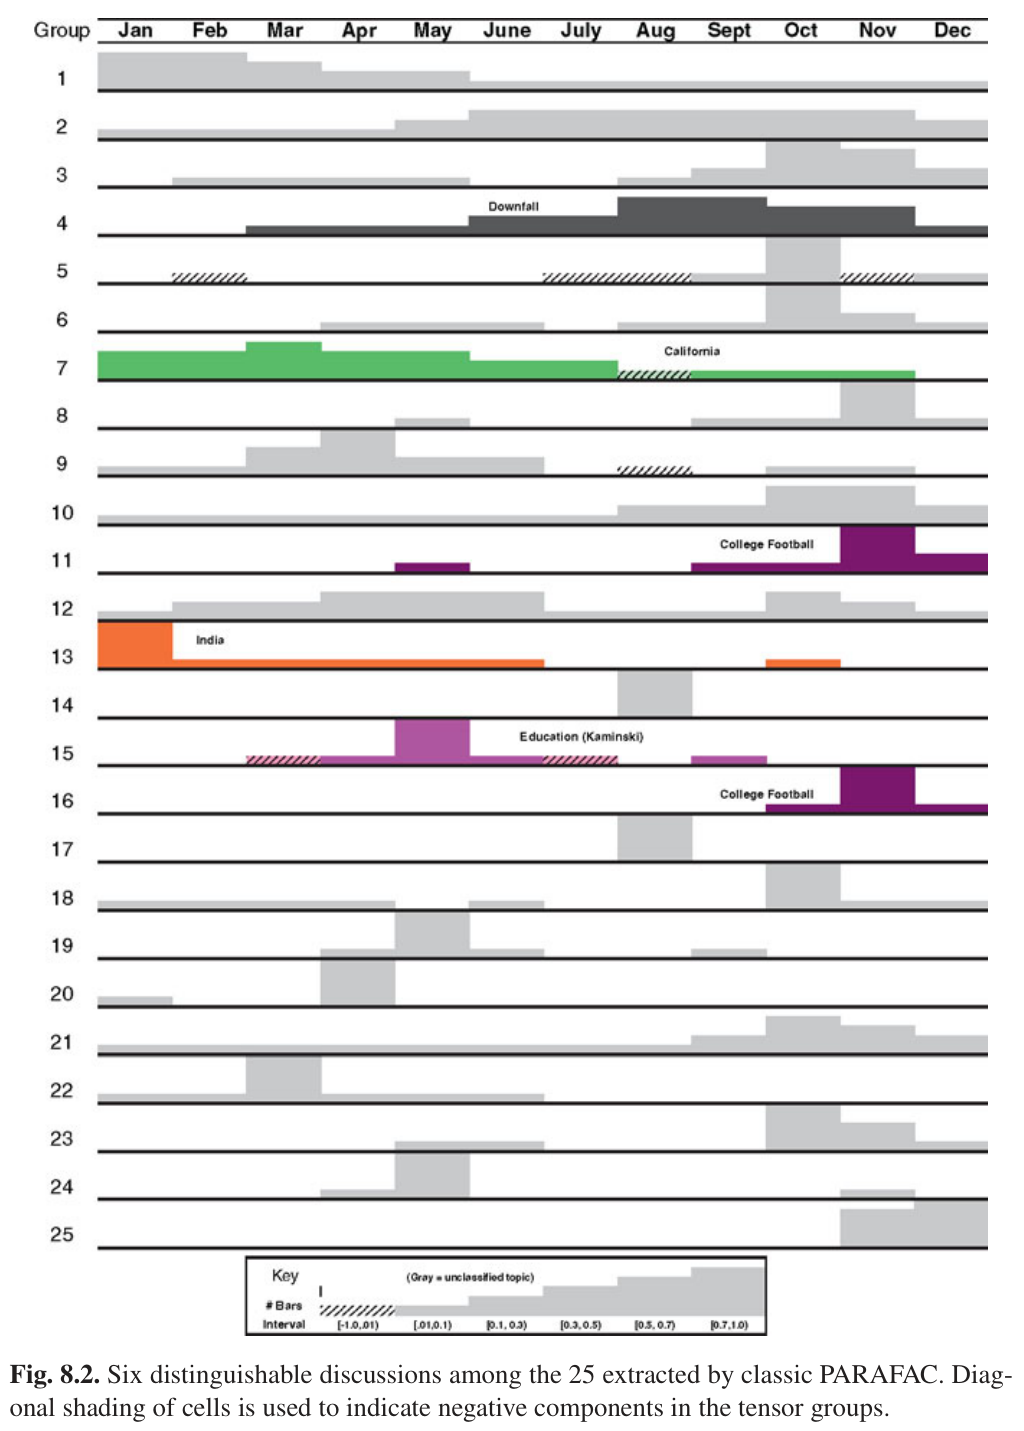
\includegraphics[max height=0.8\textheight]{images/enron-parafac}
    \end{center}
\end{frame}

\begin{frame}{Non-Negative PARAFAC Results}
    \begin{center}
    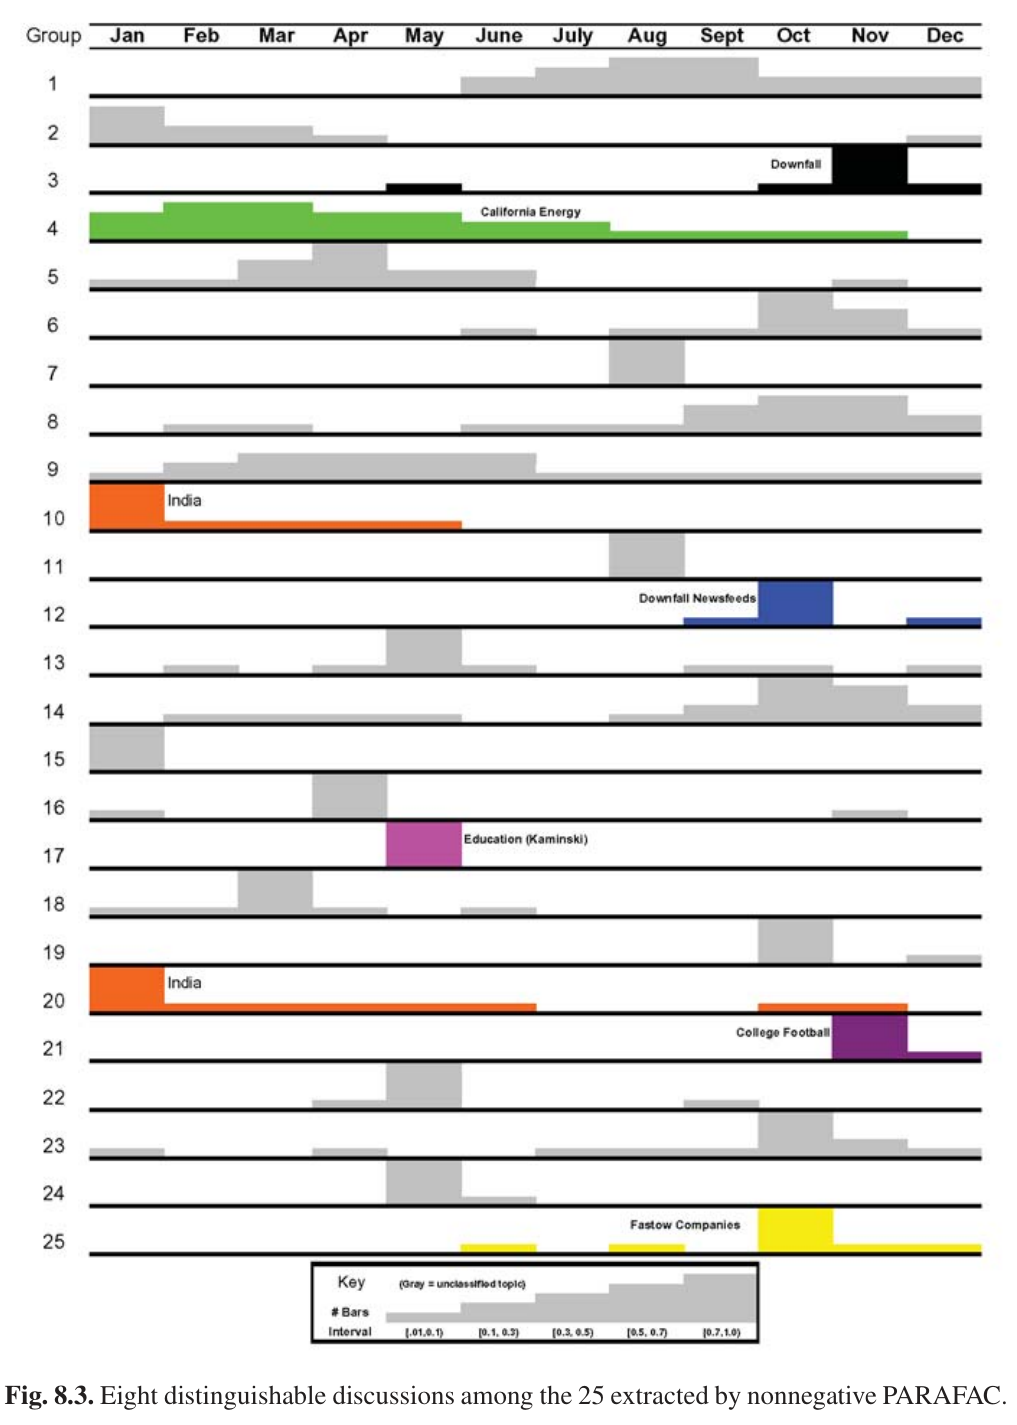
\includegraphics[max height=0.8\textheight]{images/enron-nn-parafac}
    \end{center}
\end{frame}



\end{document}